This section is focused on showing the basic preliminary results obtained. 

A short-term goal is to resolve the local positioning problem using Bayes Filter algorithm. Such algorithm has two steps: the prediction and the error correction. The first step will be creating a custom robot model on Webots, then programing a controller to move it around avoiding collision with the walls, implementing odometry techniques to determine an estimation of its position in a rectangular small arena and then creating a data set collecting sensor measurements data along with positioning in order to create a model that will allow the robot to correct the odometry data.

\section{Robot And The Environment}

In order to implement the Bayes Filter algorithm an e-puck-style robot model will be created. The main benefit to do so is the high control and personalization on the robot model that brings when running different experiments. Thus a list with the main components is given below.

\begin{itemize}
\item A \textit{cylindric body} in which all the components will be attached. 
\item Two \textit{cylindric wheels} with hinge joints, each with a position sensor and a rotational motor. The former serves to obtain the position of the wheel at a given time step, the later controls the velocity and direction of the wheel.
\item Eight \textit{laser-type distance sensors} around the body of the robot that measure the distance between the robot and the closest wall.
\item A \textit{compas} sensor for measuring the robot orientation over the virtual north.
\end{itemize}

Figure \ref{fig:ch-3:robot-view} illustrates the created custom robot model under two different views. The white cylinders are the wheels, the purple is the body, and the yellow are the distance sensors. This robot is based on the version provided by the examples of custom robot models on the Webots Documentation. It is slightly personalized, mainly on the type of distance sensors used.

\begin{figure}[h!]
  \centering
  \begin{subfigure}[b]{0.41\linewidth}
  	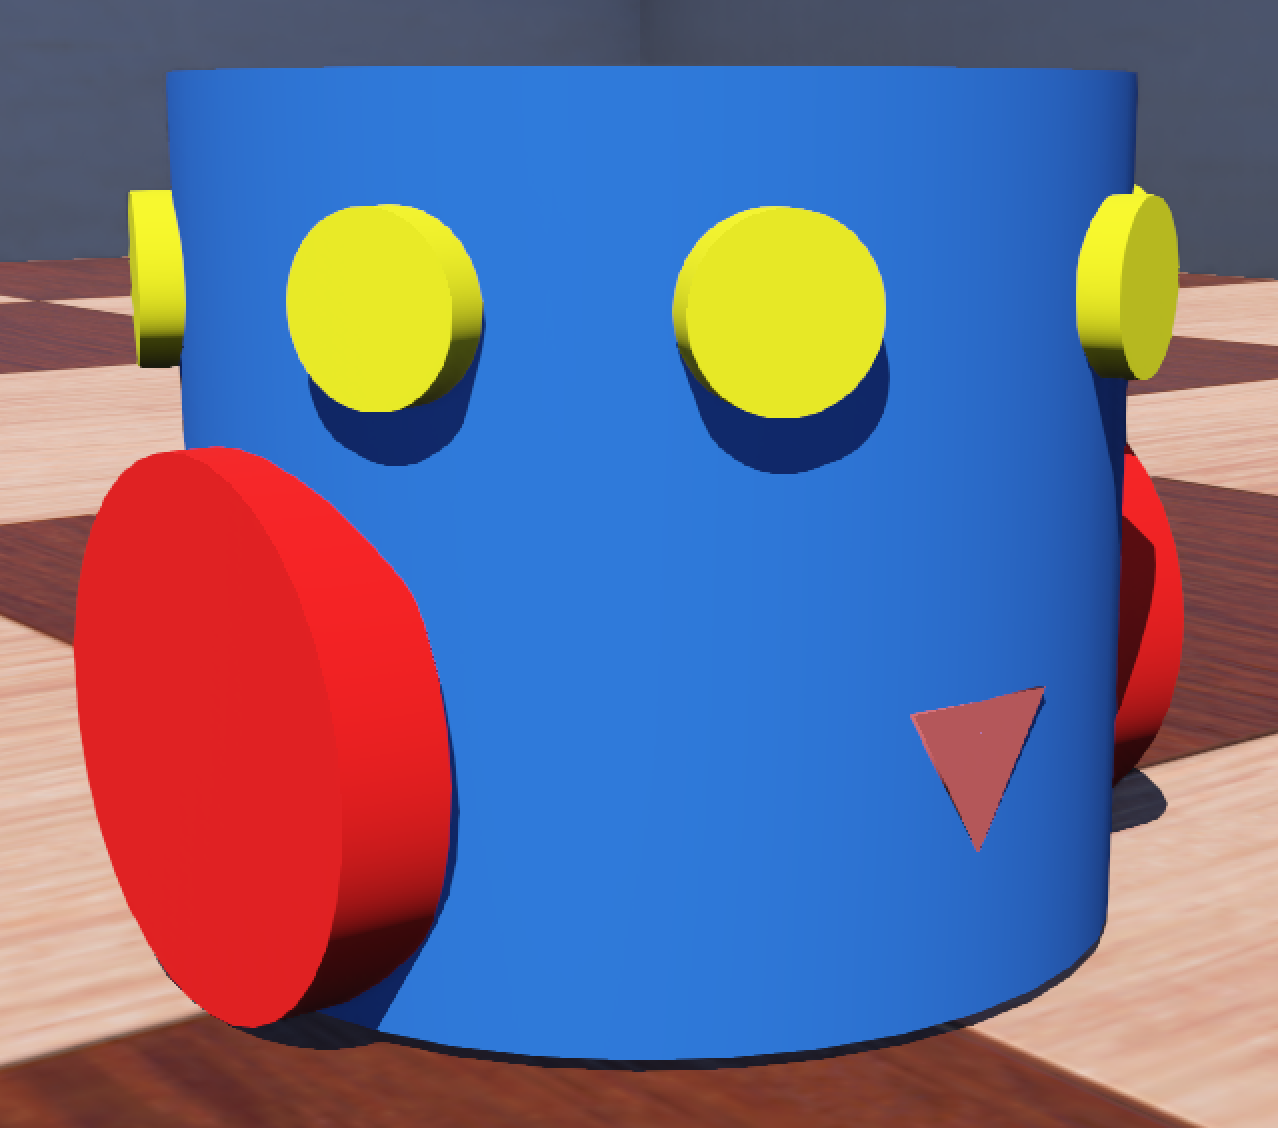
\includegraphics[width=\linewidth]{\images/chapter3/robot.png}
	\caption{Plain rendering}
  	\label{fig:ch-3:robot-1}
  \end{subfigure}
  \begin{subfigure}[b]{0.4\linewidth}
  	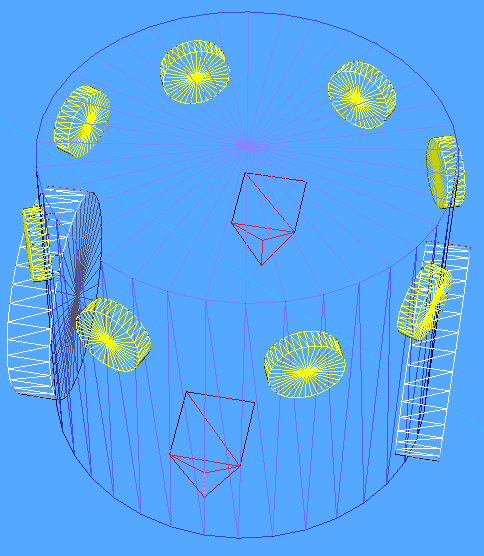
\includegraphics[width=\linewidth]{\images/chapter3/robot1.png}
	\caption{Wireframe rendering}
  	\label{fig:ch-3:robot-2}
  \end{subfigure}
  \caption{Custom robot view}
  \label{fig:ch-3:robot-view}
\end{figure}

The robot is positioned at the center of an arena of 1.5m x 2m surrounded by walls. This position is communicated to the robot and it becomes its initial state. In order to avoid obstacles while translating, a simple algorithm has been used that turns around the robot when the front sensors tell the presence of a solid object near 15 cm of distance.

\section{Pose Prediction}

Webots introduces the concept of supervisor which is a class forming part of the Webots API that simulates human actions in the environment. For instance, it can restart the simulation and put the robot in a random position or it can measure the trajectory of the robot at each step. Notice that this last concept is strictly restricted to the Webots simulator and it is not part of the command line of any real robot. Combined along with the compass sensor data will be useful to get the true state $\mathbf{x_t} = [x_t, y_t, \theta_t]^T$ where $x_t \text{ and } y_t$ are the coordinates of the robot translated to the GRF and $\theta_t$ is the orientation of the robot over the virtual north at time $t$. The predicted state will be $\mathbf{\hat{x}_{t}} = [\hat{x}_t, \hat{y}_t, \hat{\theta}_t]^T$ and it can be updated recursively based on the previous given state and thus at time $t+1$ the state will be $\mathbf{\hat{x}_{t+1}} = \mathbf{\hat{x}_{t}} + [\Delta x, \Delta y, \Delta \theta]^T$. 

Cyberbotics' Robot Curriculum website\cite{webots-curri-odometry} provides a good explanation about how to implement odometry technique and which parameters need to be calibrated in order to have a precise implementation. These parameters need to be found experimentally since they are not measurable directly with enough precision: the distance of increment for the left wheel, the right wheel and the distance between both wheels. To have those values well configured four tests need to be performed:

\begin{itemize}
\item \textit{Increments per tour: } the number of motor increments made per one complete wheel rotation. While the robot have gone forward, the wheel had made one complete tour. 
\item \textit{Axis wheel ratio: } the diameter of the wheels divided by the distance between them. The robot turns around on its own axis and the goal is to end up at the same position that it began.
\item \textit{Wheels diameters: } the robot follows a square trajectory and it should end up at the same position where it started. If that is not the case, the diameter of one wheel can differ to the other as it is shown in figure \ref{fig:ch-3:wheel-diameters}.
\item \textit{Scaling factor: } it configures the scale of the trajectory.
\end{itemize}

\begin{figure}[h!]
  \centering
  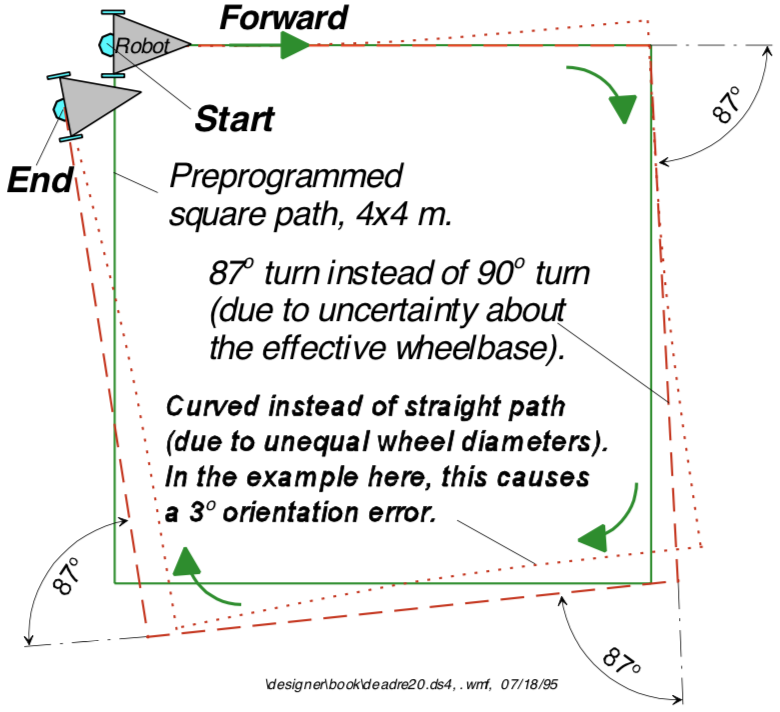
\includegraphics[width=0.6\linewidth]{\images/chapter3/wheel-diameters.png}
  \caption{Wheel diameters test.}
  \label{fig:ch-3:wheel-diameters}
  \source{Where am I?\cite{Feng:where-am-I}}
\end{figure}

After performing the tests and having an estimation of the corresponding values the results are shown in figure \ref{fig:ch-3:odometry-res}.    The plots were taken in an aerial-view way where the axis represents the width and height of the arena and the lines mark the trajectory of the robot. On the one hand the blue line represents the true state position of the robot obtained by the supervisor and compass data, on the other hand the orange line represents the estimated position of the robot using odometry techniques. The left-side image was obtained by running one simulation of the mobile robot with zero noise on its position sensors. Even though the odometry measurements approximate very well to the true pose, there is a small difference and this is due to the fact that the parameters used by odometry were found experimentally and thus some error was introduced. The odometry data quickly starts to diverge when there is certain noise associated with the position sensors as it is shown in the right-side image.

\begin{figure}[h!]
  \centering
  \begin{subfigure}[b]{0.47\linewidth}
  	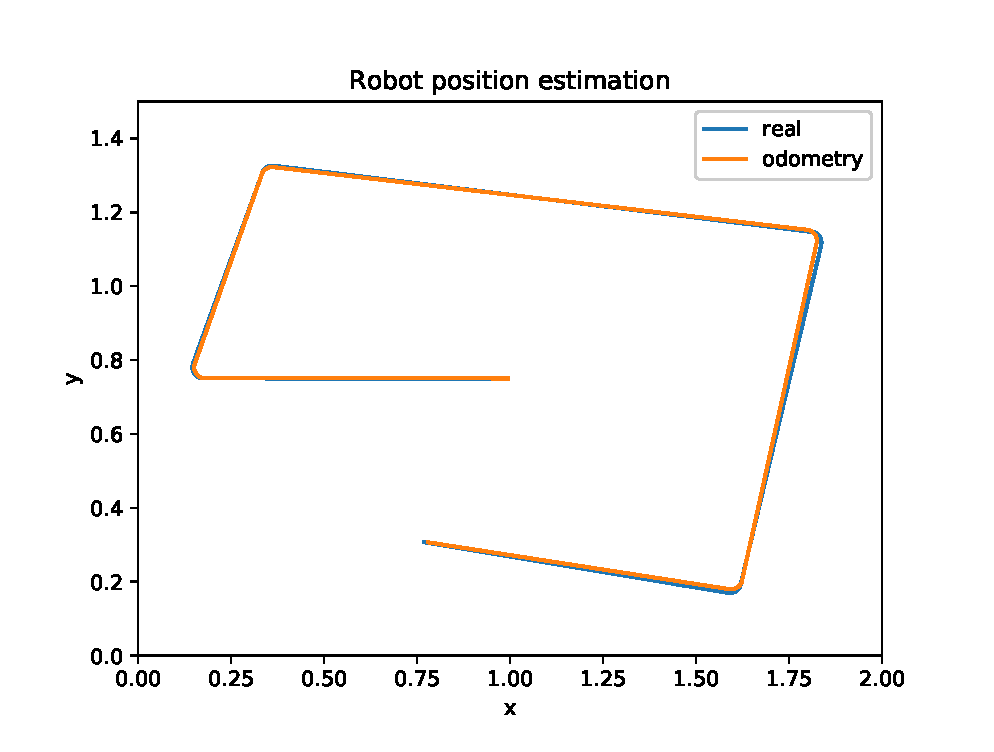
\includegraphics[width=\linewidth]{\images/chapter3/position-00-error.eps}
	\caption{Position Sensor Noise = 0}
  	\label{fig:ch-3:noise-0}
  \end{subfigure}
  \begin{subfigure}[b]{0.47\linewidth}
  	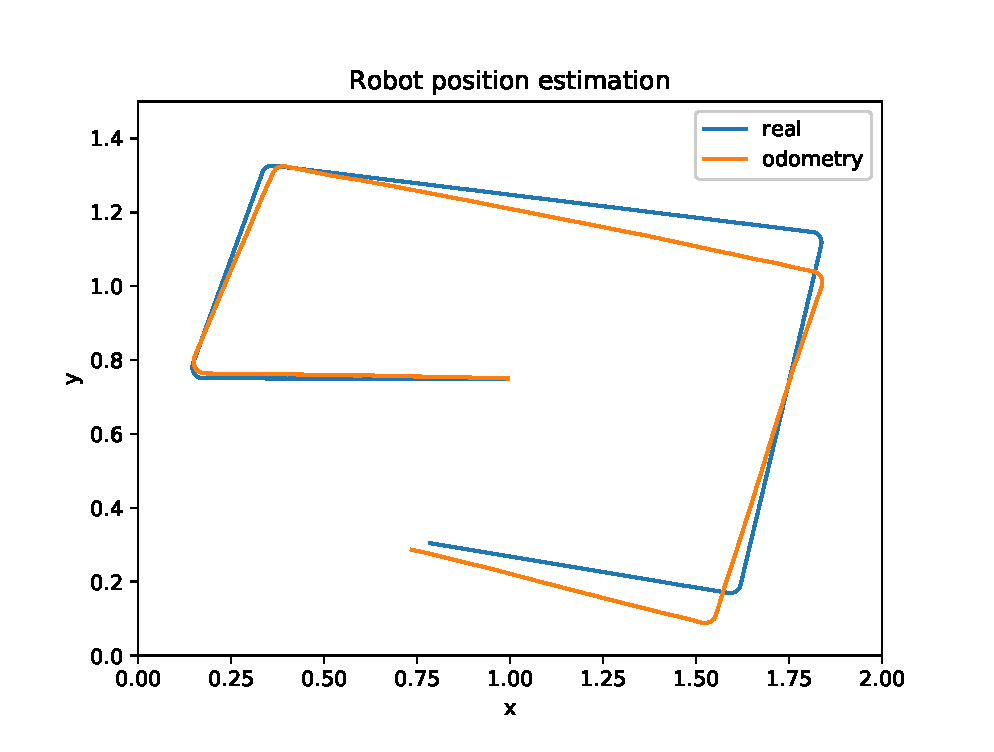
\includegraphics[width=\linewidth]{\images/chapter3/position-01-error.eps}
	\caption{Position Sensor Noise = 0.1}
  	\label{fig:ch-3:noise-1}
  \end{subfigure}
  \begin{subfigure}[b]{0.6\linewidth}
  	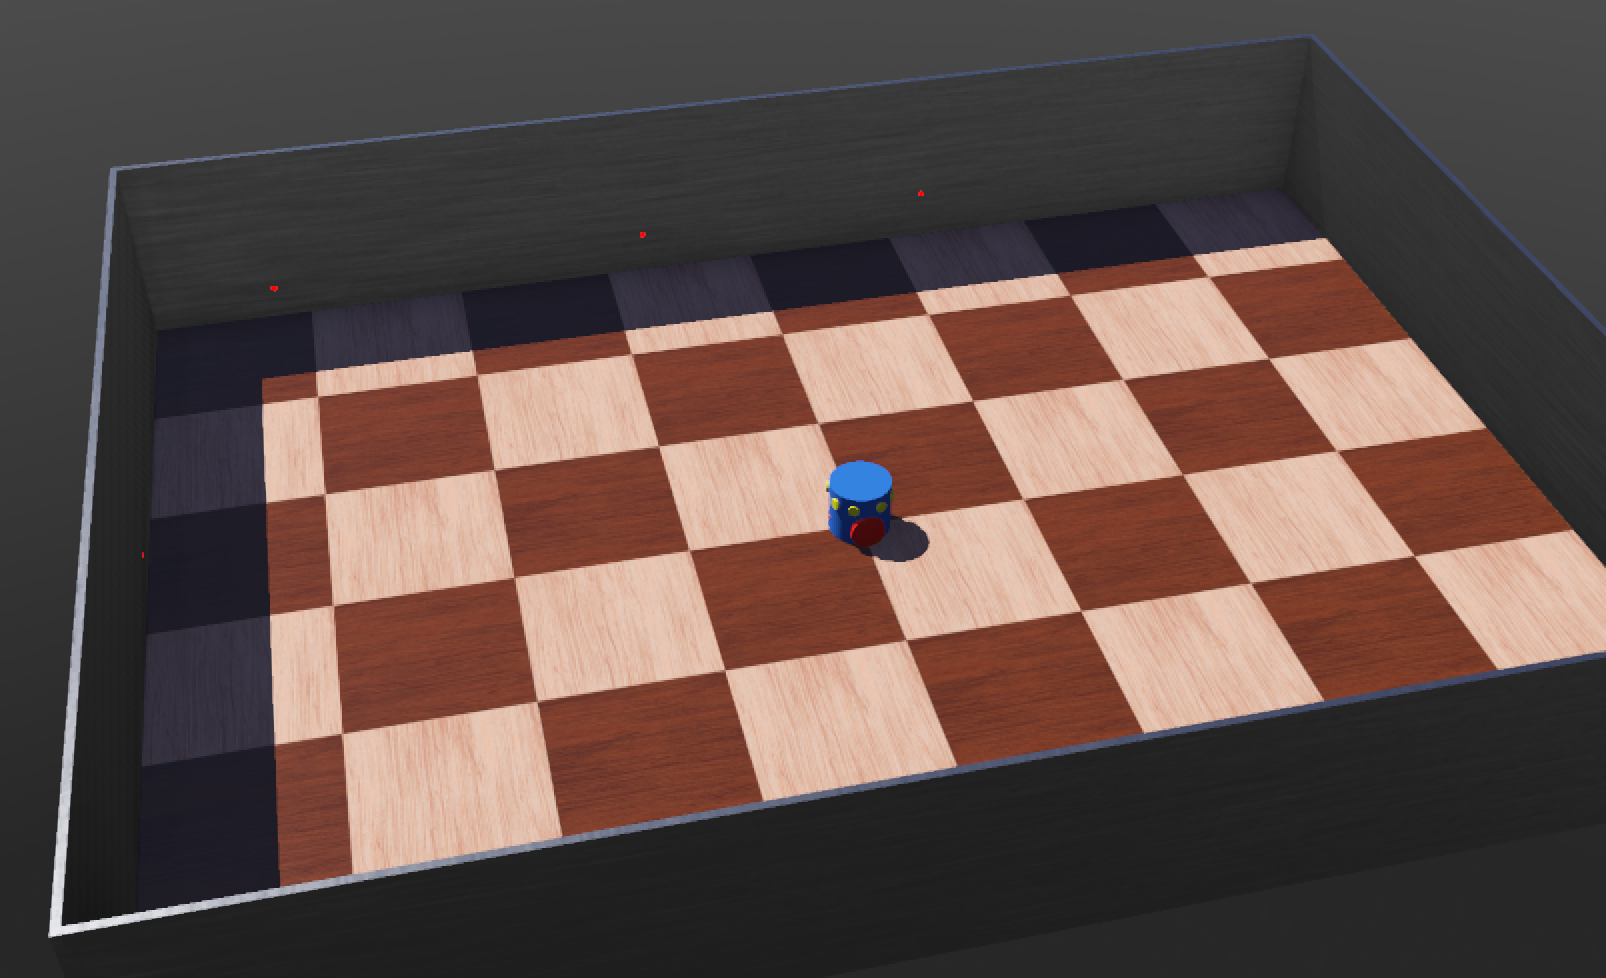
\includegraphics[width=\linewidth]{\images/chapter3/arena.png}
	\caption{Robot in the arena}
  	\label{fig:ch-3:arena}
  \end{subfigure}
  \caption{Odometry results}
  \label{fig:ch-3:odometry-res}
\end{figure}

\section{Collecting Sensor Data and Pose}

An artificial data set is constructed based on distance sensor and robot position information, the objective to do so is to generalize and predict sensor measurements over a robot pose.

First, a noise of $\pm0.1$ was introduced in the distance sensors. Second, the simulation was run during $\sim$ 10 minutes in fast mode while collecting sensor measurements of the true robot state. Furthermore some of the sensor data is missing intentionally. The data set was split in 80\% training and 20\% test. The target variables are the sensor measurements and the features are the $[x_t, y_t, \theta_t]^T$ variables for different values of $t$.  Then a random forest algorithm was used with only 10 trees to predict sensor measurements given the robot pose. Finally the accuracy of the fit is measured to be 99\%. Such high accuracy can be caused by the small-size arena since the robot could have been passed by the same place multiple times generating an overfit on the data.

\section{Pose Correction}

The pose correction is made each 450 robot steps. The idea is to take a range of state values, that is the coordinates plus the robot orientation, near the odometry data given at time $t$, for each state value obtain a prediction (using the random forest model trained before) on the distance sensor estimates and then compare them with the true sensor data. The corrected state value will be the one whose prediction better approximates to the true sensor data. An area of 20 cm for the robot coordintes and $\pm3$ degrees of range for the robot orientation are considered for each state value around the odometry data.  Figure \ref{fig:ch-3:pose-correction} shows the results. The green point represents the corrected state value and thus the odometry data is corrected at that point.

\begin{figure}[h!]
  \centering
  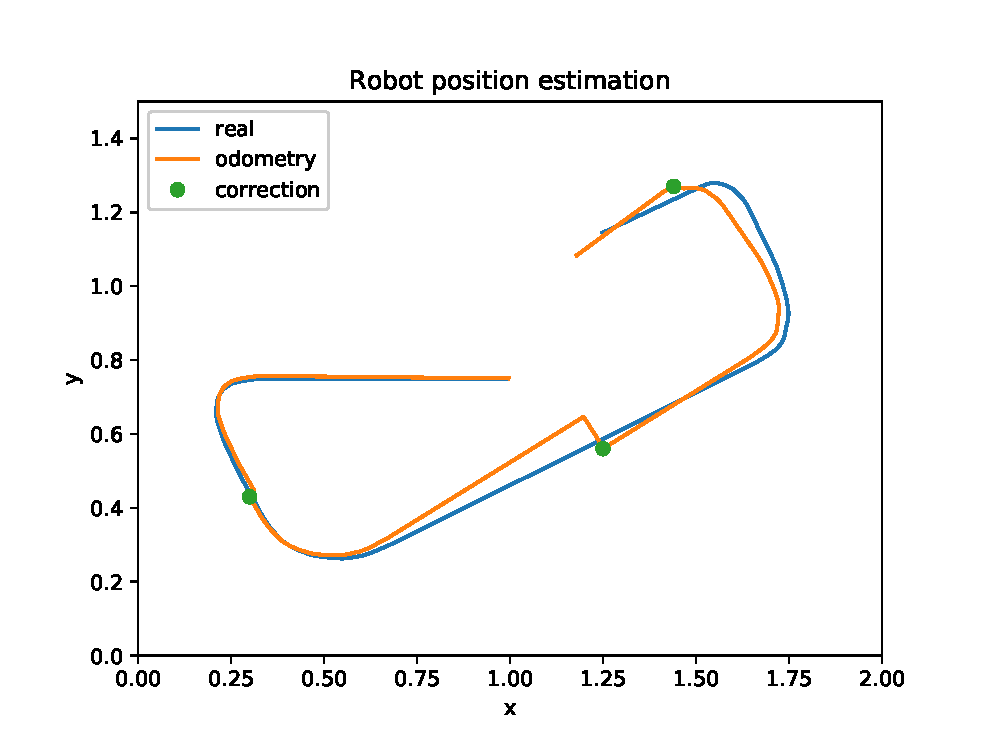
\includegraphics[width=0.7\linewidth]{\images/chapter3/position3.eps}
  \caption{Pose correction}
  \label{fig:ch-3:pose-correction}
\end{figure}

Even though the first two error corrections are very accurate, the third one is not. This can be caused because the data set used to train the model was obtained with only one run of the simulation and thus the predictions are not very accurate when the robot visits a place far from the ones visited in the data set. One solution would be to execute more simulations while collecting data and to add some more random control actions to the robot in order to obtain more covered places into the arena.

\section{Discussion and Further Work}

The implemented example represents the basic idea to the Bayes Filter algorithm. It serves as an illustrative idea but it has a poor performance since the amount of predictions needed for each correction step are enormous. Further work will lead to the error correction step using more advanced techniques as Particles Filter. Additionally some stochasticity will be added in the robot control actions that will lead to a less predictive trajectory and thus covering more regions in the arena while collecting data. Moreover the size of the arena is ideal for running simulations but real-world scenarios can be less predictive and far more complex. Thus a more realistic environment will be created.









